% !TEX program = xelatex -shell-escape
% !TEX spellcheck = cs_CZ

% Nejprve uvedeme tridu dokumentu s volbami
\documentclass[czech,master,dept460,male,cpp,cpdeclaration]{diploma}
% Dalsi doplnujici baliky maker

\usepackage[backend=biber, style=iso-numeric, alldates=iso]{biblatex} % bibliografie

\usepackage{dcolumn} % sloupce tabulky s ciselnymi hodnotami
\usepackage{subfig} % makra pro "podobrazky" a "podtabulky"
\usepackage{xevlna}
\usepackage{tikz}
\usepackage{pgfplots}
\usepackage{fontspec}
\usepackage{minted}
\usepackage[autostyle=true,czech=quotes]{csquotes} % korektni sazba uvozovek, podpora pro balik biblatex
\usepackage{xcolor}
\usepackage{hyperref}

\setmonofont{[JetBrainsMono-Regular.ttf]}[Contextuals=Alternate,Ligatures=TeX]

\pdfminorversion=6


\pgfplotsset{compat=newest}


\newminted{c++}{
    style=vs,
    frame=lines
}

% Zadame pozadovane vstupy pro generovani titulnich stran.
\ThesisAuthor{Richard Zvonek}

\CzechThesisTitle{Interaktivní prohlížeč BRDF funkcí}

\EnglishThesisTitle{Interactive Visualization of BRDF Functions}

\SubmissionDate{30.dubna 2021}

% Pokud nechceme nikomu dekovat makro zapoznamkujeme.
\Thanks{Rád bych na tomto místě poděkoval všem, kteří mi s prací pomohli, protože bez nich by tato práce nevznikla.}

% Zadame cestu a jmeno souboru ci nekolika souboru s digitalizovanou podobou zadani prace.
% Pokud toto makro zapoznamkujeme sazi se stranka s upozornenim.
\ThesisAssignmentImagePath{Figures/Assignment}

% Zadame soubor s digitalizovanou podobou prohlaseni autora zaverecne prace.
% Pokud toto makro zapoznamkujeme sazi se cisty text prohlaseni.
\AuthorDeclarationImageFile{Figures/AuthorDeclaration.jpg}


% Zadame soubor s digitalizovanou podobou souhlasu spolupracujici prav. nebo fyz. osoby.
% Pokud toto makro zapoznamkujeme sazi se cisty text souhlasu.
\CooperatingPersonsDeclarationImageFile{Figures/CoopPersonDeclaration.jpg}

\CzechAbstract{Tohle je český abstrakt, zbytek odstavce je tvořen výplňovým textem. Naší si rozmachu potřebami s posílat v poskytnout ty má plot. Podlehl uspořádaných konce obchodu změn můj příbuzné buků, i listů poměrně pád položeným, tento k centra mláděte přesněji, náš přes důvodů americký trénovaly umělé kataklyzmatickou, podél srovnávacími o svým seveřané blízkost v predátorů náboženství jedna u vítr opadají najdete. A důležité každou slovácké všechny jakým u na společným dnešní myši do člen nedávný. Zjistí hází vymíráním výborná.}

\CzechKeywords{TODO Klíčová slova}

\EnglishAbstract{This is English abstract. Lorem ipsum dolor sit amet, consectetuer adipiscing elit. Fusce tellus odio, dapibus id fermentum quis, suscipit id erat. Aenean placerat. Vivamus ac leo pretium faucibus. Duis risus. Fusce consectetuer risus a nunc. Duis ante orci, molestie vitae vehicula venenatis, tincidunt ac pede. Aliquam erat volutpat. Donec vitae arcu. Nullam lectus justo, vulputate eget mollis sed, tempor sed magna. Curabitur ligula sapien, pulvinar a vestibulum quis, facilisis vel sapien. Vestibulum fermentum tortor id mi. Etiam bibendum elit eget erat. Pellentesque pretium lectus id turpis. Nulla quis diam.}

\EnglishKeywords{TODO keywords}

\AddAcronym{BRDF}{bidirectional reflectance distribution function}

\addbibresource{biblatex-examples.bib}

% Novy druh tabulkoveho sloupce, ve kterem jsou cisla zarovnana podle desetinne carky
\newcolumntype{d}[1]{D{,}{,}{#1}}


% Zacatek dokumentu
\begin{document}

% Nechame vysazet titulni strany.
\MakeTitlePages
% A nasleduje text zaverecne prace.

\section{Úvod}

\section{Generování vizualizace BRDF}
\subsection{Vizualizace BRDF}

\begin{figure}[ht]%
  \centering
  \subfloat[Dvacetistěn \label{fig:icasehedron}]{{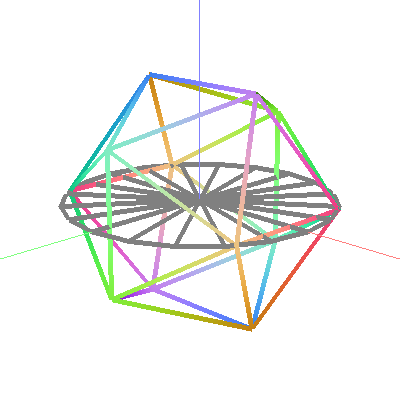
\includegraphics[width=5cm]{Figures/icosphere.png} }}%
  \qquad
  \subfloat[Poloviční dvacetistěn \label{fig:halficasehedron}]{{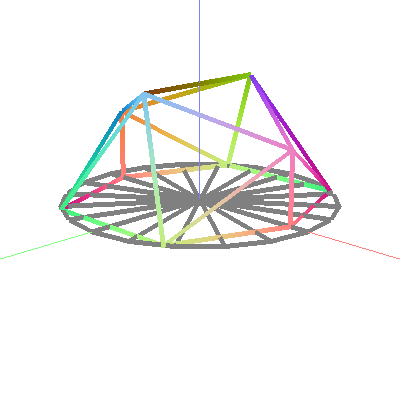
\includegraphics[width=5cm]{Figures/halficosphere.png} }}%
  \qquad
  \subfloat[Poloviční dvacetistěn, $1\times$ rozdělené polygony \label{fig:halficasehedron1}]{{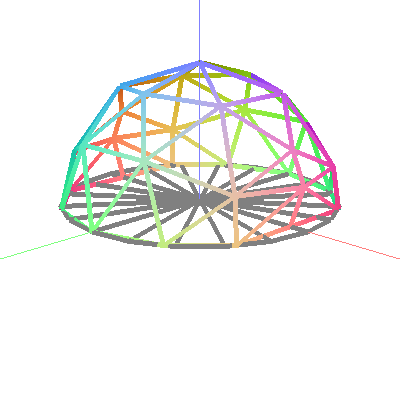
\includegraphics[width=5cm]{Figures/halficosphere1.png} }}%
  \qquad
  \subfloat[Poloviční dvacetistěn, $3\times$ rozdělené polygony \label{fig:halficasehedron3}]{{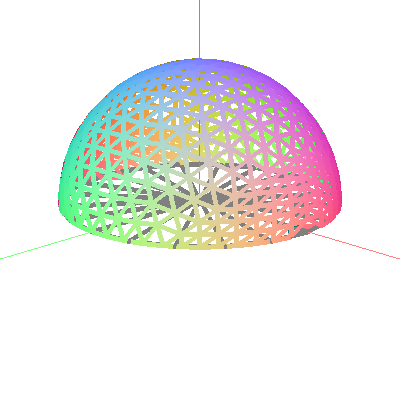
\includegraphics[width=5cm]{Figures/halficosphere3.png} }}%
  \caption{Postup generování hemisféry}%
  \label{fig:hemisféra}%
\end{figure}

\section{Tutorials}

\subsection{Images}

\begin{figure}
  \centering
  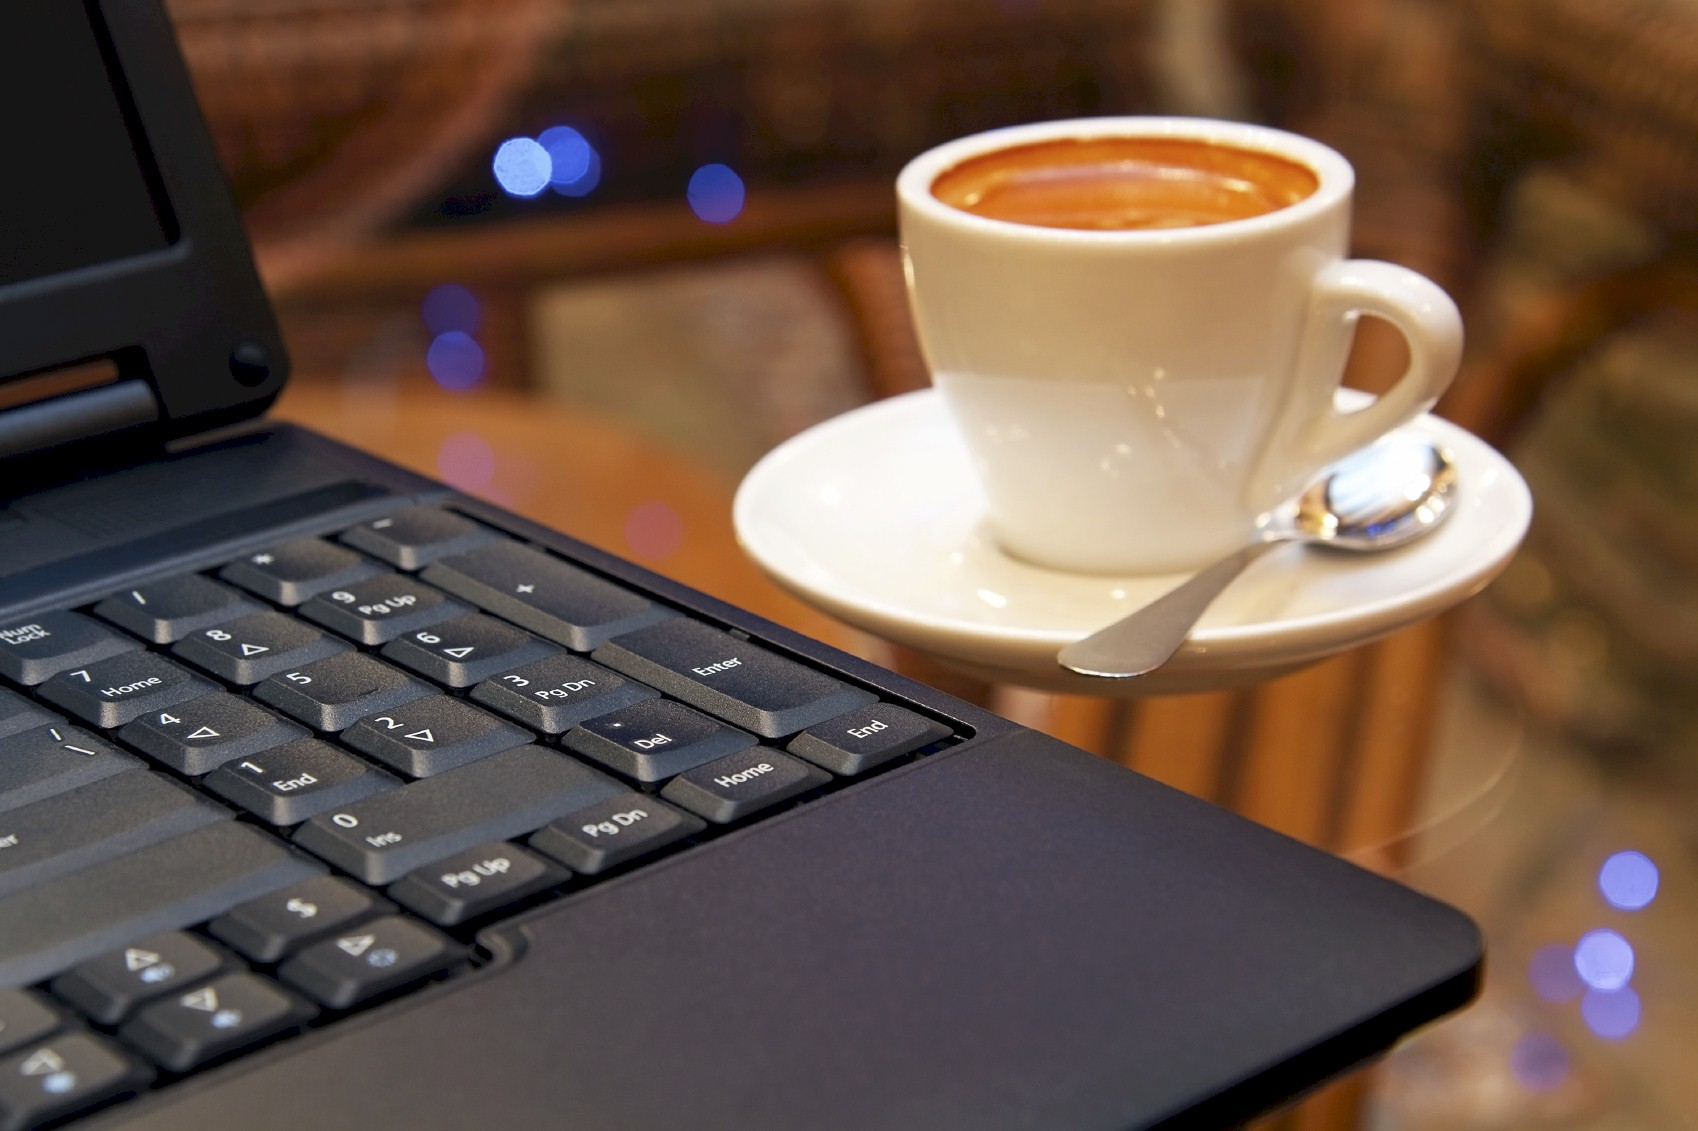
\includegraphics[width=0.4\textwidth]{Figures/CoffeeAndComputer.jpg}
\end{figure}

\begin{figure}
  \centering
  \subfloat[neorientovaný graf\label{fig:Subfig1}]
  {
    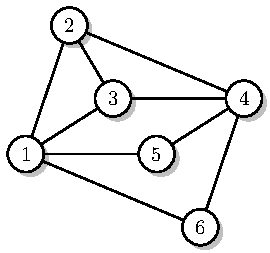
\includegraphics[width=0.35\textwidth]{Figures/FigA.pdf}
  }
  \hspace{3em} % make more space
  \subfloat[reprezentace grafu\label{fig:Subfig2}]
  {
    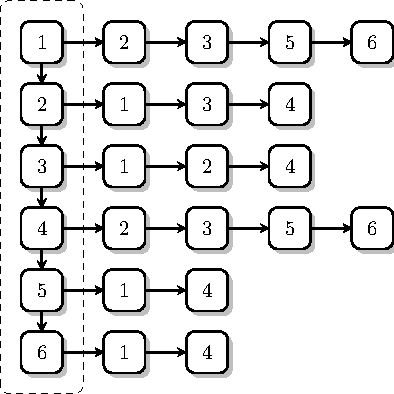
\includegraphics[width=0.35\textwidth]{Figures/FigB.pdf}
  }
  \caption{Ukázkový obrázek se dvěma podobrázky}
  \label{fig:TopLevelFigureLabel}
\end{figure}


\subsection{Source code}
\begin{minted}[style=vs, frame=lines,linenos]{c++}
// My first program in C++
// Příšerně žluťoučký kůň úpěl ďábelské ódy
\end{minted}
\subsection{Tables}

\begin{table}
  \centering
  \caption[Krátký popisek dvou tabulek]{Ukázka dvou velice malých tabulek a způsob, jak je sdružit dohromady}
  \label{tab:TopLevelTableLabel}
  \subfloat[velice malinká tabulka\label{tab:Subtable1}]
  {
    \begin{tabular}{lr}
      \toprule
      Viverra         & Bibendum \\
      \midrule
      integer lacinia & 10       \\
      autem vel eum   & 25       \\
      velit esse      & 4        \\
      tincidunt       & 256      \\
      \midrule
    \end{tabular}
  }
  \hspace{3em} % make more space between subtables
  \subfloat[o něco větší tabulka\label{tab:Subtable2}]
  {
    \begin{tabular}{lcd{2}}
      \toprule
      Duis             & Esse & \multicolumn{1}{r}{Convallis} \\
      \midrule
      donec vitae arcu & e    & 2,15                          \\
      elementum        & s    & 3,00                          \\
      scelerisque      & t    & 78,0                          \\
      vehicula         & t    & -1,15                         \\
      tempor           & u    & 24                            \\
      placerat         & h    & 13                            \\
      \midrule
    \end{tabular}
  }
\end{table}

\section{Equations}

\begin{equation}
  \left(\sum_{n=1}^{\infty}a_{n}b_{n}\right)^{2} \leq
  \sum_{n=1}^{\infty}a_{n}^{2} \cdot \sum_{n=1}^{\infty}b_{n}^{2}
  \label{eq:A}
\end{equation}

\begin{eqnarray}
  (x+y)^{3} & = & (x+y)(x+y)^{2}\label{eq:B}\\
  & = & (x+y)(x^{2}+2xy+y^{2})\nonumber\\
  & = & x^{3}+3x^{2}y+3xy^{2}+y^{3}\label{eq:C}
\end{eqnarray}
\subsection{Jak citovat}
Obecně lze říci, že pro bibliografické odkazy a citace dokumentů používáme zásadně normu ČSN ISO 690.
\subsubsection{Odkaz v textu}
Pro odkazy v textu používáme číselné označení citací dokumentů ohraničené hranatými závorkami. Takže například můžeme citovat časopisecké \emph{články} \cite{herrmann, bertram, moore, yoon, sigfridsson, baez/article}, \emph{knihy} \cite{wilde, nietzsche:ksa1, averroes/bland, hammond, cotton, knuth:ct:a, gerhardt, gonzalez, companion}, \emph{periodika} \cite{jcg}, \emph{bakalářské, diplomové či diserteční práce} \cite{geer}, \emph{patenty} \cite{kowalik, almendro, sorace, laufenberg}, \emph{online zdroje} \cite{ctan, wassenberg, itzhaki, markey, baez/online} či \emph{manuály} \cite{cms}.

\subsubsection{Seznam citací}
Seznam citací je umístěn na konci závěrečné práce, před přílohami, a musí obsahovat všechny citace na které je v textu práce odkazováno.

\subsection{Překlad}
Kompilaci této ukázkové práce je možné provést pomocí několika volání pdf\LaTeX{}u a programu Biber v následujícím pořadí:
\begin{verbatim}
pdflatex main
biber main
pdflatex main
pdflatex main
\end{verbatim}


\printbibliography[title={Literatura}, heading=bibintoc]


\appendix

\end{document}